\documentclass[11pt]{article}
\setlength{\textwidth}{6.3in}
\setlength{\textheight}{9in}
\setlength{\oddsidemargin}{0in}
\setlength{\evensidemargin}{0in}
\setlength{\topmargin}{-.6in}
\linespread{1.3}

% \renewcommand{\labelenumi}{\alph{enumi}}
\usepackage{epsfig}
\usepackage{amsmath}
\usepackage{amssymb}
\usepackage{amsfonts}
\usepackage{tikz}
\newcommand{\spacer}{\displaystyle{\phantom{\int}}}
\newcommand{\blank}[1]{\underline{\hspace{#1}}}
\newenvironment{piecewise}{\left\{\begin{array}{l@{,\quad}l}}{\end{array}\right.}
\newcommand{\points}[1]{({\it #1 points})}
\hyphenation{}

\graphicspath{ {./}{../figures/} }

\begin{document}
\noindent \textbf{Sam Voisin \hfill  \textbf{Topological Data Analysis: Class Project}  \hfill  December 11, 2019} \\
\line(1,0){455}

\begin{center}
\Large{{\bf Gesture Recognition via Electromyograph Signals}}\\
\end{center}

\begin{enumerate}
\setlength{\parindent}{5ex}

\item \textbf{Introduction}

\noindent

Skeletal muscles produce electrical activity known as \emph{myoelectric impulses} upon contraction. These myoelectric impulses can be detected and recorded using an electromyograph (EMG). EMGs are currently used to study a number of neuromuscular conditions.

Two electromyograph categories exist currently. The first type of EMG, introduced in 1950, is the \emph{intramuscular EMG}. The intramuscular EMG uses subcutaneous sensors implanted in the skeletal muscle through thin wires. The second EMG type is the \emph{Surface} electromyograph ("sEMG"). The sEMG uses sets of two or more electrodes placed on the surface of the skin. The sEMG  represents a compromise between the invasive nature and greater precision associated with its intramuscular counterpart. 

Superficial qualities of the subject being measured can have a detrimental affect on the quality of sensor readings. Some examples of these qualities are perspiration, body-fat content, or shifting of sensor pads \cite{lobov}.

A more recent technology trend is that of wearable technology or \emph{wearables} \cite{wear}. Modern wearables typically perform a variety of tasks including providing information such as text message alerts and capturing biological data such as the user's heart rate. Wearables have been depicted in SciFi novels and movies for decades but have only recently become common to consumers. As discussed in section 3, quality wearable devices combined with reliable and cost-effective myoelectric sensing technology may lead to a new generation of intuitive human-computer interface ("HCI") devices.

\item \textbf{Problem Statement}

As sEMG devices decline in size and cost, they have become a focus for researchers interested in the information they might provide.The problem of classifying motion as captured with sEMG sensors is not a new one. Researchers have published articles as early as 1967. Indeed, the number of publications on the topic has grown considerably in the last 20 years \cite{state}. In particular, the problem of classifying movements is now popular enough that several datasets of recorded signals and subject characteristics have been generated and published \cite{ninapro}.

As stated above, there have been many successful attempts to classify gestures  using EMG sensor data. Common methods employed to this task are linear discriminant analysis, artificial neural networks, support-vector machines and more \cite{state}. Despite this success, consumers have been slow to adopt HCI devices for a number of reasons. Two major factors represent hurdles to continued advances in this area:
\begin{enumerate}
\item[1)] Limited computational resources - Available processing power and on-board memory are restricted to what can be embedded in a necessarily low-profile device. The artificial neural network ("ANN") is a prime example of a high-performing algorithm that has performed will in-sample but does not generalize well due to these constraints.

\item[2)] Availability of training data - The amount of training data required to achieve satisfactory results without overfitting is limited to the quality and configuration of equipment of a single study \cite{bigdata}. While the NinaPro database offers a number of relevant data to be used in training gestures classifiers, the data is generated across differing experiments where test subjects make differing gestures while wearing sensor arrays in differing configurations. As a result, the amount of available training data is not linear in the number of new studies being performed.
\end{enumerate}

This project seeks determine whether it is possible to identify latent features common to various classes of gestures while removing variance associated with superficial qualities of the test subject and minor differences in quality and configuration of the sEMG sensor array. The figure 1 depicts a proposed data pipeline for this purpose.

\begin{figure}[h]
\centering
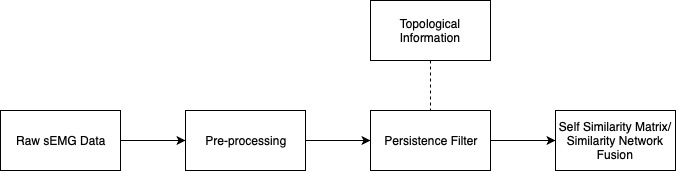
\includegraphics[width=0.75\textwidth]{pipeline}
\caption{Proposed data pipeline}
\end{figure}

This pipeline consists of two primary components:
\begin{enumerate}
\item[1)] A filtering component capable of remove superficial noise inessential to classifying gestures.
\item[2)] A classification component capable of identifying a gesture. Ideally this classification will be performed as early as possible in the gesture cycle.
\end{enumerate}
Hypotheses, testing, and construction of these components are described in greater detail in section 4. If the suggested pipeline is feasible, training data captured across studies may be utilized in classification with minimal information loss.

\item \textbf{Previous Work}

The primary work that inspired this project is  \emph{Latent Factors Limiting the Performance of sEMG-Interfaces} by Lobov, \emph{et al.} \cite{lobov}. The research team in this study set out to train both a linear discriminant analysis ("LDA") classifier and an artificial neural network ("ANN") classifier capable of identifying gestures. The classifier would then be used to assist users in playing a simple game via the \emph{Myohalmic armband}, a wearable HCI device equipped an sEMG sensor array. Subjects were able to control the game with some success using gestures. However, performance was far better when using a mouse or joystick. The sEMG training data was smoothed using a root mean square (RMS) moving average.

More recently, Phinyomark \emph{et al.} found applications of TDA for EMG data similar to those generated in \cite{lobov}. They sampled overlapping windows of EMG signals and then reduced the dimension of these windows via principal component analysis. The \emph{mapper} algorithm was applied to the resulting vectors to create a topological network representing the feature space of EMG signals. Signal amplitude and power, nonlinear complexity and frequency information, and time-series structure were determined to be the most influential features for identifying gesture patterns \cite{topograph}.

The preferred classifier to be utilized in the pipeline in figure 1 utilizes self-similarity matrices ("SSMs") and is based on the similarity network fusion ("SNF") method described in \cite{snf}. As a brief summary, SSMs are symmetric matrices whose entries represent a measure of similarity between two points in a time-ordered point cloud ("TOPC"). This measure of similarity may be a distance metric such as the $L_2$ distance or a similarity measure like the gaussian kernel. A set of SSMs generated from differing signal sources can be normalized and thought of as a transition matrix which can be utilized to randomly walk over a connected graph representing the TOPC. If sufficient iterations are performed, a stationary distribution will be reached and the resulting matrix will also be a similarity matrix which captures information from all of the individual matrices. This approach to clustering seems appropriate to the problem at hand because it was developed to handle sensor data generated from differing sources much like the 8 sensors in my data set (section 3). Additionally, this technique does not need the large, homogeneous training data sets required to adequately fit ANNs or other models with large parameter sets. In the paper, the authors use the SNF method on 2 and 3 modalities. My project attempts the method with 5. As we will see, this is a resource intensive endeavor.

\newpage

\item \textbf{Data}

The \emph{EMG data for gestures Data Set} from the UCI Machine Learning Repository \cite{uci} was utilized for this project. This data set was collected by Lobov, \emph{et al.} to conduct research for \cite{lobov}.

This data set consists of 36 subjects performing a series of six distinct gestures. Four of these gestures are simple motions including moving the hand up, down, left, or right (figure 2). The final two motions are complex motions created by a combination of two simple motions (e.g. moving the hadn up and to the left simultaneously).

\begin{figure}[h]
\centering
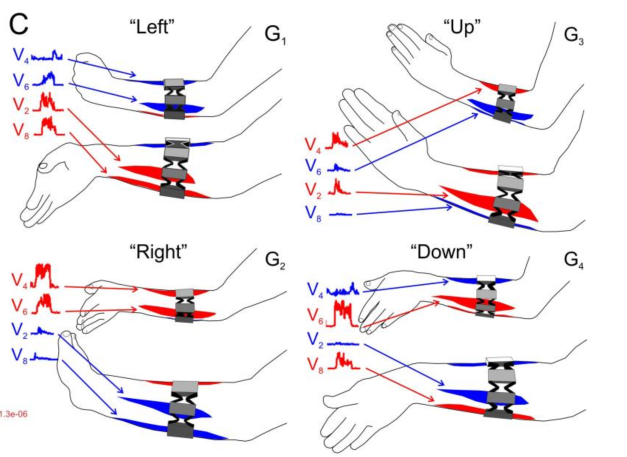
\includegraphics[width=0.5\textwidth]{gests}
\caption{Simple gestures captured by Lobov \emph{et al.} \cite{lobov}}
\end{figure}

Subjects performed all gestures four times for approximately 1.5 to 3 seconds for each. The motions were captured by a MyoThalmic bracelet placed as depicted in figure 2. Of the eight evenly spaced sensors, five were situated directly on five main muscles - \emph{flexor carpi radialis}, \emph{flexor carpi ulanis} \emph{extensor carpi radialis longus}, \emph{extensor digitorum}, \emph{extensor carpi ulanis}, \emph{flexor}, and \emph{palmaris longus}.

To make computation more tractible only the five primary channels were considered in constructing the proposed pipleline (figure 1). Similarly the two complex gestures were removed from the dataset leaving only the four simple gestures. The result is a data set of approximately 720 matrices of size $t \times 6$. The 7 columns of each matrix are time (in milliseconds), sensor readings 2 4, 5, 6, and 8, and a gesture label column.

A notable data issue discovered during exploratory analysis is a large disparity in the amount of time that each subject performed their gesutres. Some subjects performed gestures for close to the full $3s$ asked of them. However, it was much more common for a subject to perform a gesture for approx. $2s$ while some subjects performed a gesture for as little as $1.7s$. Another issue with the dataset is imprecision in the sEMG sensors used. Signals registered in by the MyoThalmic bracelet are truncated towards their peaks and troughs. However, the dataset continues to include readings during the peak and trough periods using the last recorded value. Curves with very "blocky" appearaces are the result (figure 3).

\begin{figure}[h]
\centering
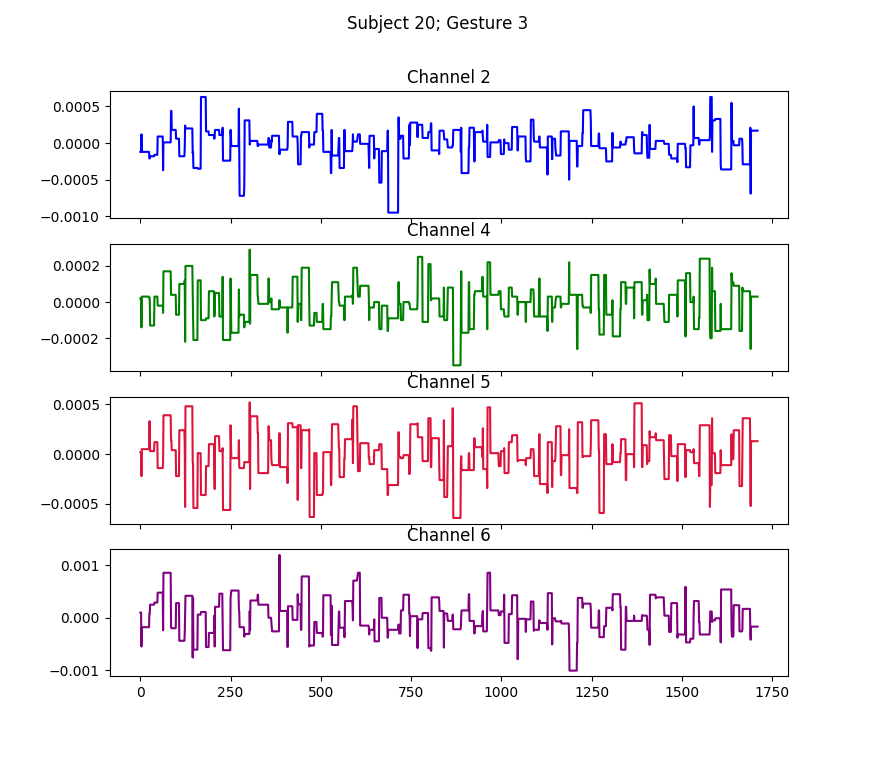
\includegraphics[width=0.75\textwidth]{s20g3}
\caption{Subject 20 gesture 3. Duration ($ms$) is on the horizontal axis.}
\end{figure}

\item \textbf{Analysis Methods}

\begin{enumerate}
\item[1)] \textit{Constructing the Filtering Mechanism}

The first step in constructing a filtering mechanism was determining features that were informative with regards to the gesture being performed. A $20 \times 20$ persistence image was generated with a spread parameter of $\sigma = 1\times 10^{-5}$ over the surface formed by the 5 sEMG channels. This was performed for all 720 simple gestures. the $20 \times 20$ pixel parameter was chosen for modeling purposes described below. The spread parameter was chosen to enusre some identifiability remained between gestures. Some samples of these persistence images are deicted below (figure 4). Only the $H1$ homology class is considered for computability purposes.

\begin{figure}[h]
\centering
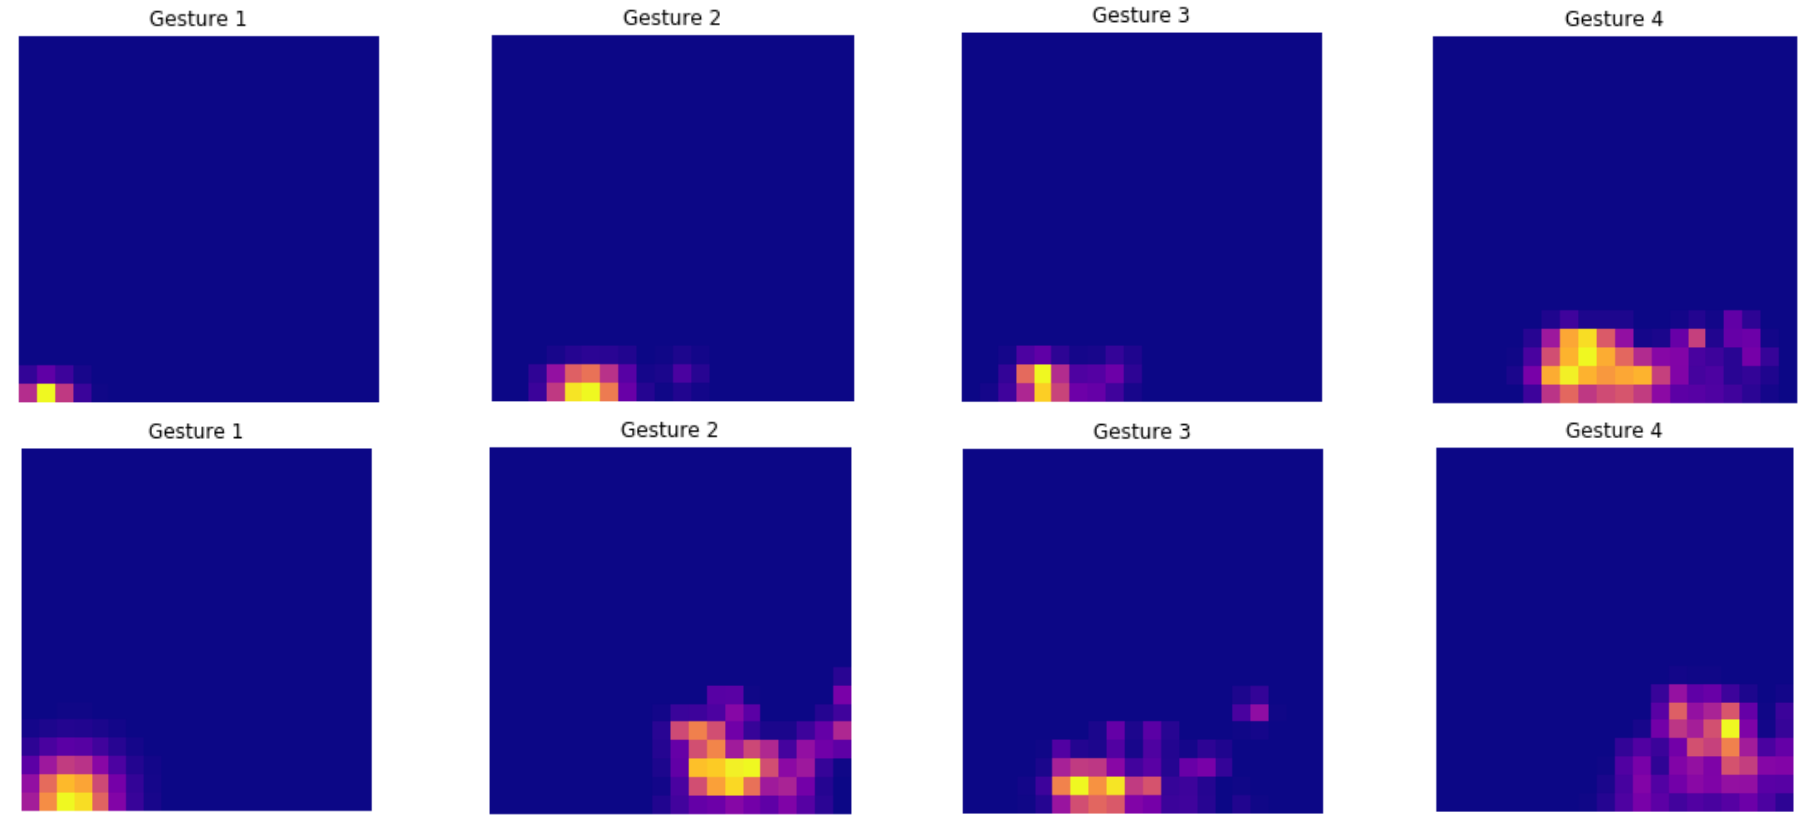
\includegraphics[width=0.75\textwidth]{persim_smpl}
\caption{Two samples of persistences images for each gesture}
\end{figure}

\newpage

As a first step in determining which features are important and which can be removed from the data, the persistence image vectors were normalized, added within their gesture classes, and the resulting vectors were normalized again. This provides a sort of empirical distribtion within ech gesture class. The resulting images are depicted in figure 5.

\begin{figure}[h]
\centering
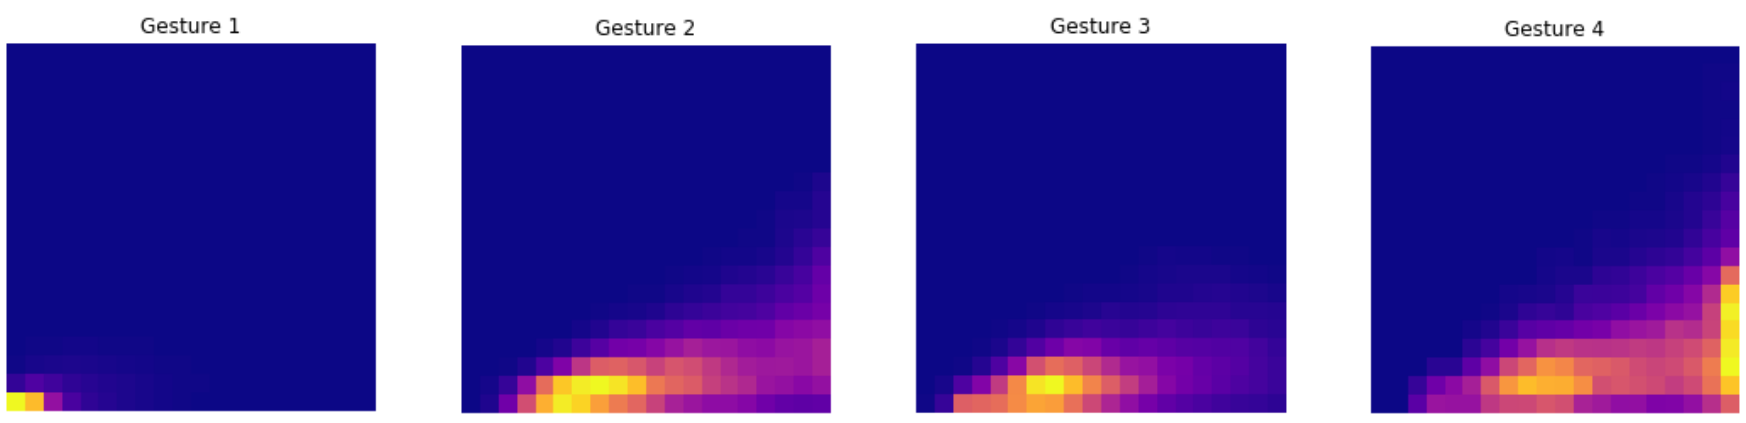
\includegraphics[width=0.75\textwidth]{comb_pims}
\caption{Normalized combinations of persistence images for each gesture}
\end{figure}

Interestingly, when used to classify the gestures by their persistence images, $57.1\%$ in-sample accuracy was achieved. This is surprisingly high for a heuristic approach to classification as they expected accuracy for a random guess is only $25\%$. However, this classifier is very fragile. Because some subjects contribute more to the sum total, when single subject is left out of the fitting process this heurisitc classifier may have $0\%$ for all of that individual subject's gestures. Alternatively, some subjects were fit with perfect accuracy when left out of the training sample. This provides evidence that commonalities do exist across subjects with regards to gesture performance.

The approach just described is interesting, but determining important features requires a more rigorous approach. This rigor is achieved by applying an $L_1$ normalized multi-class logistic regression to the persistence images. The $L_1$ penalty is included in order to achieve a more sparse set of parameters with the hopes of creating a more aggressive filter. The inverse persistence images formed by the regression coefficients (one for each of the 400 pixels) are arranged and presented below.

\begin{figure}[h]
\centering
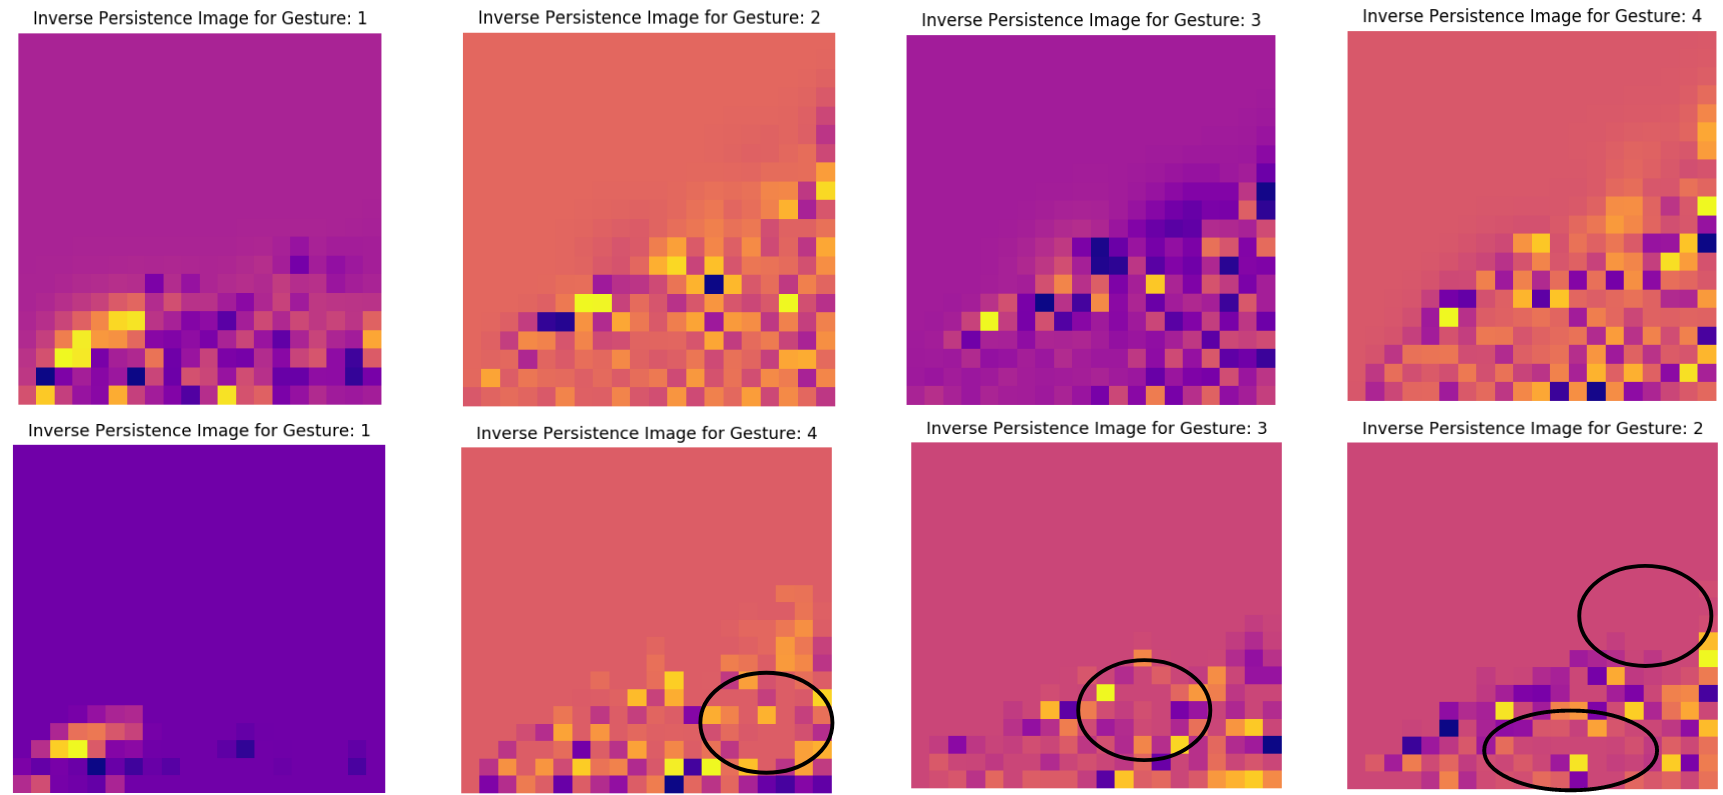
\includegraphics[width=0.75\textwidth]{inv_persims}
\caption{Inverse persistence images of non-sparse (top row) \& sparse (bottom row) regression coefficients}
\end{figure}

From figure 6 we can see that the sparsity induced by the $L_1$ penalty is mostly induced in the middle and high persistence $1$-cycles. This discovery represents a problem for the construction of a persistence filter because it shows that the information provided by the low persistence $1$ cycles is important to retain. Because of the elder rule, we cannot remove more persistent cycles without also removing those cycles with also removing less persistent cycles.

It is possible that by inlcuding the full gesture cycle, as opposed to just the beginning or just the end of the cycle, information about \emph{two} gestures has been included - the motion to make the gesture and the motion caused by releasing the gesture and returning to a neutral state. This may have a sort of "mirror image" effect making gestures more challenging to recognize. Further research will be done to test this hypothesis as well as to determine commonalities among gestures which are misclassified by the regression models.

\item[2)] \textit{Constructing the Classifier}

As discussed in section 2, the preferred classifier for the pipeline is a self-similarity template for each of the relevant gestures. A Self-Similarity class was created in python for this purpose. This class is capable of taking in a time ordered point cloud with an arbitrary number of modalities as an array are returning a series of SSMs combined into a single $t \times t \times m$ tensor. Each SSM is constructed using a prespecified similarity measure. A number of SSMs were created with varying similarity measures. Figure 7 depicts SSMs for subject 10 performing gesture 2 twice and subject 20 performing gesture 2 once. Channels 2, 4, and 5 are presented here.

\begin{figure}[h]
\centering
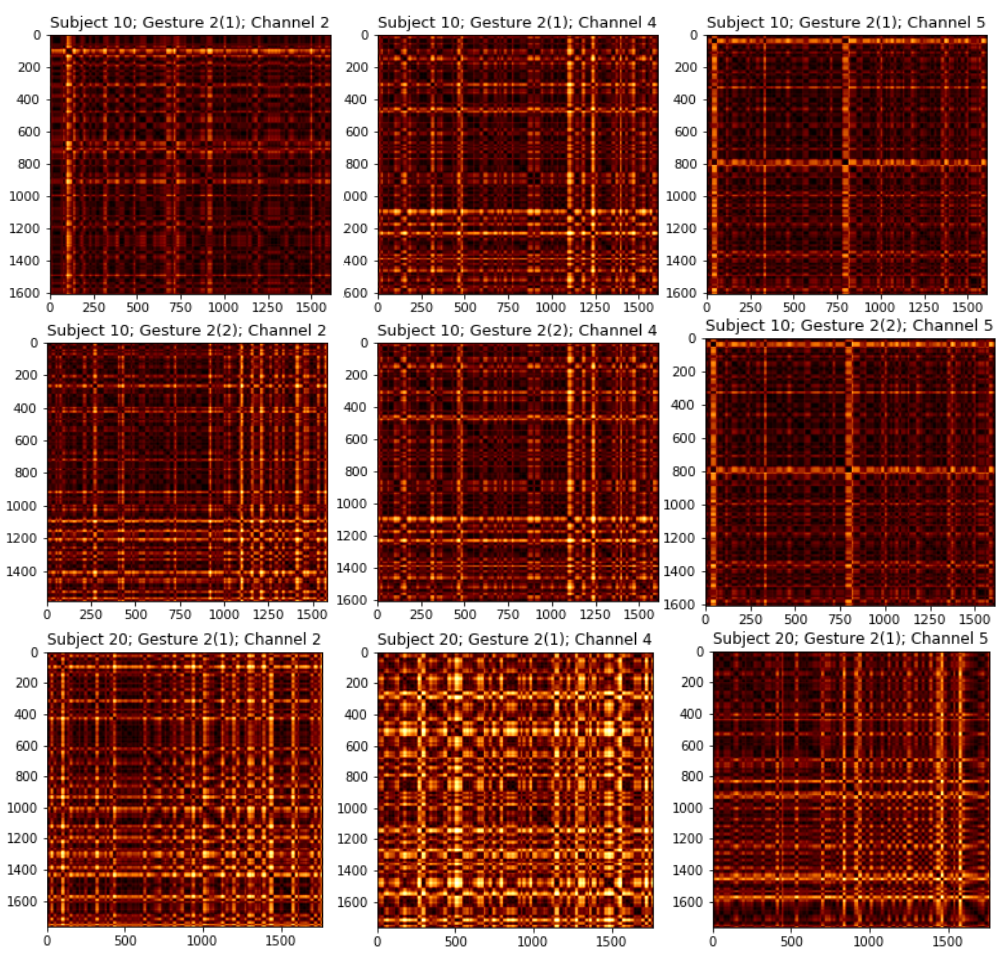
\includegraphics[width=0.75\textwidth]{all_ssm}
\caption{SSMs generated by gestures from subjects 10 \& 20.}
\end{figure}

\newpage

Clear similarities can be seen when comparing the two iterations of the gesture performed by subject 10. However, there is considerable between-subject variability with regards to the SSMs. This variability is present between many other subjects beyond the two examples presented here. Notable, there are some subjects whose SSMs exhibit similar characteristics for the same gesture. There is still reason to believe that a latent structure exists between subjects.

As stated in section 4 (Data), there are many instances of subjects performing their gestures for imprecise periods of time. This requires the use of a method known as \emph{dynamic time-warping} \cite{dtw}. Dynamic time-warping is an algorithm capable of finding optimal matches in the peaks and troughs between two time-series data sets. This technique has been applied to similar problems in the past and should be a solution to the problems described here. Unfortunately, due to computing resource constraints and the size of the data set at hand, performing dynamic-time warping was not feasible. The algorithm for dynamic time-warping has complexity $\mathcal{O}(n^2)$. As stated previously, $n$ ranges between 1,500 and 3,000 for a single modality. This prevented conclusive work on constructing self-similarity templates. Plans for mitigating these issues are described in the following section.

\end{enumerate}


\item \textbf{Next Steps}

Several modifications must be made to the analysis steps described above in order to obtain conclusive results and continue the construction of the classification pipleline:

First, computing resources capable of performing the memory and time intesnive tehcniques required for dynamic time-warping and similarity network fusion. This represents the primary bottleneck to classification. Fortunately, Duke University makes several resources available for these types of projects through their compute cluster service. The computational burden can be futher reduced by more sparsely sampling the modalities. The data points are currently very densely sampled and redundant. Many of these points can likely be removed without issue.

Second, on the topic of constucting a persistence filter, it may be more appropriate to use sliding window 1-D persistence ("SW1Pers") to analyze important features in the sEMG signals data. Some work using SW1Pers has already been performed; however, additional efforts to tune the sliding window parameters are needed.

Finally, it may be wise to seperate each gesture into "begin", "hold", and "release" phases. This can be used to determine whether there is indeed a "mirror image" effect (see sect. 5) causing persistence images to be difficult to classify. Determining when each phase begins and ends will be challenging as there are no labels for this.


\item \textbf{Conclusion}

The experiments described above for generating the gesture recognition pipeline have provided null results. However, they have also provided insight into the nature of the variance within and between the subjects in our data set with regards to gesture performance. Further, additoonal research questions have been raised which may lead to development of the desired gesture classifier. There exist many additional methods, including those found in topological data analysis, that can answer these questions.


\end{enumerate}

\begin{center}
\noindent\rule{16cm}{0.4pt}
\end{center}

\newpage

\begin{thebibliography}{5}

\bibitem{lobov} Lobov, Sergey, et al. “Latent Factors Limiting the Performance of sEMG-Interfaces.” Sensors, vol. 18, no. 4, June 2018, p. 1122., doi:10.3390/s18041122.

\bibitem{wear} Tehrani, Kiana, and Andrew Michael. “Wearable Technology and Wearable Devices: Everything You Need to Know.” Wearable Devices Magazine, WearableDevices.com, March 2014. Web.

\bibitem{state} Peerdeman  B,  Boere  D,  Witteveen  H,  Huis  in  ‘t  Veld  R,  Hermens H, Stramigioli S, Rietman H, Veltink P, Misra S. Myoelectric  forearm  prostheses:  State  of  the  art  from  a  user-centered perspective. J Rehabil Res Dev. 2011;48(6): 719–38. DOI:10.1682/JRRD.2010.08.016

\bibitem{ninapro} Atzori, M.et al.Electromyography data for non-invasive naturally-controlled robotic hand prostheses.Sci. Data1:140053 doi: 10.1038/sdata.2014.53 (2014).

\bibitem{bigdata} Phinyomark, A.; Scheme, E. EMG Pattern Recognition in the Era of Big Data and Deep Learning. Big Data Cogn. Comput. 2018, 2, 21. 

\bibitem{topograph} Phinyomark Angkoon, Khushaba Rami N., Ibáñez-Marcelo Esther, Patania Alice, Scheme Erik and Petri Giovanni Navigating features: a topologically informed chart of electromyographic features space14J. R. Soc. Interface

\bibitem{ssm1} Tralie, Christopher J., et al. “Geometric Cross-Modal Comparison of Heterogeneous Sensor Data.” 2018 IEEE Aerospace Conference, 2018, doi:10.1109/aero.2018.8396789.

\bibitem{snf} Tralie, Bendich, \& Harer. “Multi-Scale Geometric Summaries for Similarity-Based Sensor Fusion.” 2019 IEEE Aerospace Conference, 2019, doi:10.1109/aero.2019.8741399.

\bibitem{dtw} Holt, G.A., et al. “Gesture Recognition Using Skeleton Data with Weighted Dynamic Time Warping.” Proceedings of the International Conference on Computer Vision Theory and Applications, 2013, doi:10.5220/0004217606200625.

\bibitem{uci} “EMG Data for Gestures Data Set.” UCI Machine Learning Repository: EMG Data for Gestures Data Set, https://archive.ics.uci.edu/ml/datasets/EMG data for gestures.

\end{thebibliography}
  
\end{document}
